\documentclass{standalone}
\usepackage{tikz}
\usepackage{pgfplots}

\begin{document}

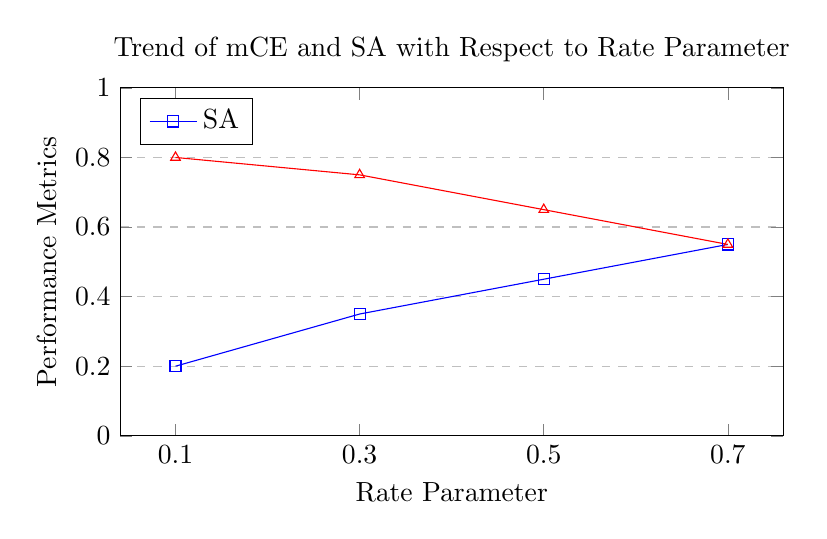
\begin{tikzpicture}
    \begin{axis}[
        title={Trend of mCE and SA with Respect to Rate Parameter},
        xlabel={Rate Parameter},
        ylabel={Performance Metrics},
        ymin=0,
        ymax=1,
        legend pos=north west,
        ymajorgrids=true,
        grid style=dashed,
        width=10cm,
        height=6cm,
        xtick=data,
        ]
        
        % Placeholder data for Mean Calibration Error (mCE)
        \addplot[blue, mark=square] coordinates {(0.1, 0.2) (0.3, 0.35) (0.5, 0.45) (0.7, 0.55)};
        \legend{mCE};
        
        % Placeholder data for Structural Accuracy (SA)
        \addplot[red, mark=triangle] coordinates {(0.1, 0.8) (0.3, 0.75) (0.5, 0.65) (0.7, 0.55)};
        \legend{SA};
        
    \end{axis}
\end{tikzpicture}

\end{document}